% !TEX TS-program = pdflatex
% !TEX encoding = UTF-8 Unicode

% This is a simple template for a LaTeX document using the "article" class.
% See "book", "report", "letter" for other types of document.

%%%%%%%%%%%%%%%%%%%%%%%%%%%%%%%%%%%%%
%
% Template para producir documentos "camera ready" para Anales de la AFA
% 
%  No se debería tener que modificar nada del siguiente preámbulo, donde están 
%  las customizaciones para adaptar la clase "article" a los Anales AFA.
%
%%%%%%%%%%%%%%%%%%%%%%%%%%%%%%%%%%%%%
\documentclass[10pt,twocolumn]{article} 

\usepackage[utf8]{inputenc} % set input encoding (not needed with XeLaTeX)
\usepackage[spanish]{babel}
\usepackage{amsmath}
\usepackage{float}


%%% DIMENSIONES DE LA PÁGINA
\usepackage{geometry} 
\geometry{a4paper} 
 \geometry{top=2.25cm} 
 \geometry{bottom=2.25cm} 
 \geometry{left=2cm} 
 \geometry{right=2cm} 


%%% PACKAGES
\usepackage{placeins}
\usepackage{graphicx} 
\usepackage{paralist} % very flexible & customisable lists (eg. enumerate/itemize, etc.)
\usepackage{verbatim} % adds environment for commenting out blocks of text & for better verbatim
\usepackage{subfig} % make it possible to include more than one captioned figure/table in a single float
\usepackage{lipsum}  
\usepackage[superscript]{cite}  %REFERENCIAS EN SUPERÍNDICE
\usepackage{hyperref}

\hypersetup{
    colorlinks=true,
    linkcolor=black,
    citecolor=black
}

% Ajusta los captions de tablas y figuras a italics
\usepackage[format=plain,
            labelfont=it,
            textfont=it]{caption}
% These packages are all incorporated in the memoir class to one degree or another...

%%% HEADERS & FOOTERS
\usepackage{fancyhdr} % This should be set AFTER setting up the page geometry
\pagestyle{fancy} % options: empty , plain , fancy
\renewcommand{\headrulewidth}{0pt} % customise the layout...
\lhead{}\chead{}\rhead{}
\lfoot{}\cfoot{\thepage}\rfoot{}
%\renewcommand{\thefootnote}{\fnsymbol{footnote}}

\usepackage{varwidth}
\usepackage{authblk}
\newcommand{\filiacion}[2]{\affil[#1]{\protect\begin{varwidth}[t]{\linewidth}\protect\centering \normalfont#2 \protect\end{varwidth}}}
\newcommand{\autor}[2]{\author[#1]{\bf #2}}
\newcommand{\corresponding}[2]{\author[#1]{\bf #2\thanks{}}}
\newcommand\cauthemail[1]{\footnotetext{#1}}
\newcommand{\fecha}[1]{\date{\vspace{-1ex}\small{#1}}}
\newcommand{\firstpagelogos}{%
  \noindent\makebox[\textwidth][c]{
\includegraphics[width=3.35cm]{figuras/logos.png}}\par
  \vspace*{-0.15cm}%
}
\date{}  % Empty date command
\renewcommand\Authand{, }
\renewcommand\Authands{, }
\newcommand{\titulo}[2]{%
  \title{%
    \bf{\large{#1%
    \if\relax\detokenize{#2}\relax
    \else\\ \vspace{1.5ex} #2%
    \fi}}}}
\newcommand{\esresumen}[1]{\small{#1 \par}\vspace{1.5ex}}
\newcommand{\pclaves}[1]{\small{\emph{#1} \par}\vspace{1.5ex}}
\newcommand{\enresumen}[1]{\small{#1 \par}\vspace{1.5ex}}
\newcommand{\keywords}[1]{\small{\emph{#1} \par}\vspace{1.5ex}}



%%% APARIENCIA DE TITULOS, SECCIONES Y SUBSECCIONES
\usepackage{titlesec}
\titleformat{\section}
  {\fontsize{10}{12}\selectfont\sffamily\bfseries\upshape}
  {\thesection}{0.6em}{}
\titleformat{\subsection}
  {\fontsize{10}{12}\selectfont\sffamily\bfseries\upshape}
  {}{0pt}{}
\titlespacing*{\section}{0pt}{1.5ex}{0.8ex}
\titlespacing*{\subsection}{0pt}{1.2ex}{0.6ex}
\setcounter{secnumdepth}{1}   %no numera las subsecciones

\usepackage[nottoc,notlof,notlot]{tocbibind} % Put the bibliography in the ToC
\usepackage[titles,subfigure]{tocloft} % Alter the style of the Table of Contents
\renewcommand{\cftsecfont}{\rmfamily\mdseries\upshape}
\renewcommand{\cftsecpagefont}{\rmfamily\mdseries\upshape} % No bold!
\renewcommand\thesection{\Roman{section}}
\renewcommand\thesubsection{}



%%% PARA EL FORMATO DE TABLAS
\usepackage{booktabs} % for much better looking tables
\usepackage{array} % for better arrays (eg matrices) in maths
\makeatletter
\newcommand{\thickhline}{%
    \noalign {\ifnum 0=`}\fi \hrule height 1.5pt
    \futurelet \reserved@a \@xhline
}
\newcolumntype{"}{@{\hskip\tabcolsep\vrule width 1pt\hskip\tabcolsep}}
\makeatother
\newcolumntype{L}[1]{>{\raggedright\let\newline\\\arraybackslash\hspace{0pt}}m{#1}}
\newcolumntype{C}[1]{>{\centering\let\newline\\\arraybackslash\hspace{0pt}}m{#1}}
\newcolumntype{R}[1]{>{\raggedleft\let\newline\\\arraybackslash\hspace{0pt}}m{#1}}

\renewcommand\spanishtablename{Tabla}  

% Corresponding author
\makeatletter
\renewcommand\@biblabel[1]{#1.}
\makeatother

\pagestyle{empty}

%%%%%% En principio no debería hacer falta modificar nada por encima de esta línea

%%%%%%%%%%%%%%%%%%%%%%%%%%%%%%%%%%%%%%%

%%% El contenido del documento comienza a partir de acá 

%título del trabajo: en el primer campo en castellano, en el segundo en inglés

\titulo{Rutas Argentinas}{} %cambiar

\autor{*}{ Nájera, Jeremías; Agost, Ignacio Raimundo}


\filiacion{*}{Física Experimental III, Instituto Balseiro\\
Centro Atómico Bariloche, Comisión Nacional de Energía Atómica\\
Universidad Nacional de Cuyo, San Carlos de Bariloche, Argentina}
\fecha{14 de marzo de 2026}

\setcounter{Maxaffil}{0}
\renewcommand\Authfont{\normalsize}
\renewcommand\Affilfont{\itshape\footnotesize}


\begin{document}

\renewcommand{\abstractname}{}
\twocolumn[
  \begin{@twocolumnfalse}
   \firstpagelogos
   \maketitle
    \begin{abstract}\vspace{-12ex}
\centering\begin{minipage}{\dimexpr\paperwidth-6cm}

\vspace{20pt}

\esresumen{
Se estudió ...
}


\end{minipage}
\vspace{4ex}
 \end{abstract}
  \end{@twocolumnfalse}
]

\thispagestyle{empty}

\iffalse
\begin{figure}[htb]
\centering
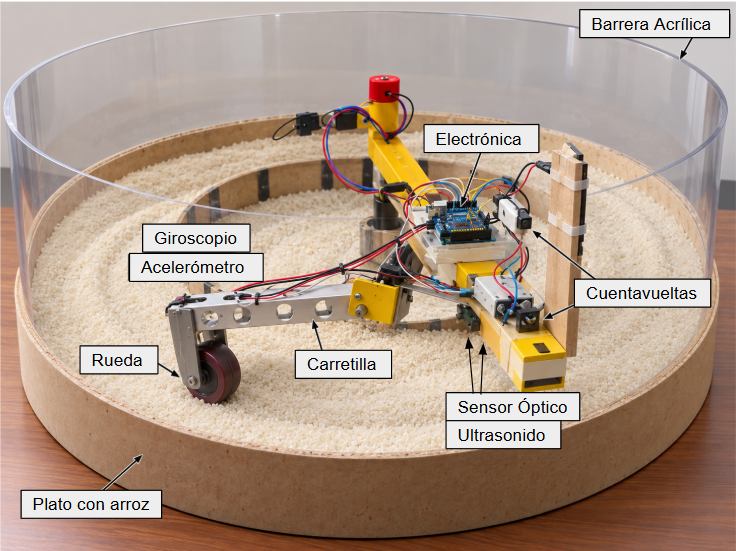
\includegraphics[width=0.82\linewidth]{figuras/esquema_experimental.png}
\caption{Esquema experimental}
\label{fig:esquema_experimental}
\end{figure}
\fi

\section{INTRODUCCIÓN}




\FloatBarrier


\section{M\'ETODOS Y MATERIALES}

\FloatBarrier


\iffalse

\begin{table}[H]
\centering
\small
\begin{tabular}{c c c c}
\hline
Relacion & $k_{ij}$ & $A_i \epsilon \sigma$ & $\sigma$ \\ \hline
$C1$-$C2$ & $0.135 \pm 0.021$ & $4.4 \pm 0.6$ & $3.9 \pm 0.6$ \\
$C2$-$C3$ & $0.0264 \pm 0.0013$ & $9.74 \pm 0.05$ & $4.44 \pm 0.06$ \\ \hline
\end{tabular}
\caption{Parametros obtenidos a partir de los ajustes lineales reducidos. Para
estimar $\sigma$ se adopto
$\epsilon = 0.94 \pm 0.01$. Unidades:
$k_{ij}$ en $\mathrm{W\,K^{-1}}$, $A_i \epsilon \sigma$ en
$10^{-10}\,\mathrm{W\,K^{-4}}$ y $\sigma$ en
$10^{-8}\,\mathrm{W\,m^{-2}\,K^{-4}}$.}
\label{tab:res-26-02}
\end{table}

\fi

\section{RESULTADOS Y DISCUSION}


\FloatBarrier

% \iffalse
\section{DISCUSION}
La limitacion del experimento realizado es que solo podemos obtener el valor de
$\epsilon \cdot \sigma$. Con lo cual, si queremos usar el resultado para estimar
alguno de estos parametros, es necesario obtener el valor del otro a partir de
otra experiencia.

\subsection*{Calculo de sigma a partir de una emisividad tabulada}
ver comentario en el codigo
% amigo no le veo nada de sentido a hacer este.
% Ese alguien calculo ese epsilon en funcion del sigma tabulado y sus mediciones.
% Si nuestro resultado tiene error, calcular algo con ese valor va a tener doblemente error.
% Calculemos el epsilon y lo comparemos con el epsilon de ese alguien y veamos por que da tanto mas chico.
% No se cual decis vos.

\subsection*{Calculo de la emisividad a partir de sigma tabulado}
Tomando como referencia el valor tabulado
$\sigma = 5.670374 \cdot 10^{-8}\,\mathrm{W\,m^{-2}\,K^{-4}}$, los valores de
emisividad $\epsilon$ inferidos se resumen en la tabla \ref{tab:epsilon}.

\begin{table}
    \begin{center}
        \begin{tabular}{| c | c |}
            relacion & $\epsilon$ \\ \hline
            C1 - C2 & $0.65 \pm 0.09$ \\
            C2 - C3 & $0.735 \pm 0.007$ \\ \hline
        \end{tabular}
        \caption{Valores de $\epsilon$ obtenidos a partir de los ajustes realizados.}
        \label{tab:epsilon}
    \end{center}
\end{table}

Estos valores son demasiado bajos y no son comparables con el valor nominal
0.97 asignado a la pintura negra mate en informes previos de Gatto y
Z\'u\~niga\cite{gatto}. Al combinar en cuadratura la incerteza
instrumental con la del ajuste, las estimaciones de $\sigma$ para las relaciones
$C2$-$C3$ quedan limitadas en buena medida por la propagacion instrumental,
mientras que en $C1$-$C2$ sigue dominando la dispersion del ajuste. La
diferencia en los valores que involucran al cilindro 1, en particular la
mostrada en el grafico \ref{fig:fit12}, puede deberse a una falla en el
termometro utilizado para el cilindro 1 o en algun punto del circuito. Sin
embargo, la relacion entre los cilindros 2 y 3 tampoco da un valor de
emisividad cercano, asi que tambien es posible que se haya da\~nado la pintura de
los cilindros, que los cilindros no sean equivalentes o que algun valor usado
en el procedimiento no haya sido bien medido.
\fi

\section{DISCUSION}
 

% \FloatBarrier

\section{CONCLUSION}

Se logró medir blablabla


\vspace{10pt}


\begin{thebibliography}{9}

\bibitem{Taberlet}
N Taberlet, S. W. Morris, J. N. McElwaine
\textit{Washboard road: The dynamics of Granular Ripples Formed by Rolling Wheels},
2007.

% \bibitem{bergman}
% T. L. Bergman, A. S. Lavine, F. P. Incropera, D. P. DeWitt,
% \textit{Fundamentals of Heat and Mass Transfer},
% 7th ed.

% \bibitem{pasco}
% PASCO, 
% \textit{Microwave Optics System — Manual WA-9314B}, 
% 2012.

% \bibitem{gatto}
% M. Gatto, J. Zúñiga,
% \textit{Determinación de constante de Stefan-Boltzmann mediante estudio de transferencia de calor por radiación},
% 2023.

% \bibitem{krossler}
% M. Krossler, J. S. Cruz,
% \textit{Determinaci\'on de la Constante de Stefan-Boltzmann mediante
% Transferencia Radiativa en un Sistema de Cilindros Conc\'entricos al Vac\'io},
% 2025.

\end{thebibliography}

\end{document}
